\documentclass{beamer}


\usepackage{graphicx}
\usepackage{amsmath}
\usepackage{algorithm}
\usepackage{algorithmic}


\author{Damien DELPY}
\title{Implementation of a Self-Organizing Map}
\institute{ENSEIRB-MATMECA}


\renewcommand{\normalsize}{\fontsize{6}{12}\selectfont}

\setbeamertemplate{footline}{%
	\hfill\insertframenumber/\inserttotalframenumber
}


\begin{document}


\begin{frame}
	
	\titlepage
\end{frame}


\begin{frame}

	\tableofcontents[sectionstyle=show,subsectionstyle=show/shaded/hide,subsectionstyle=show/shaded/hide]
\end{frame}

	

\section{Overview}
	
	\begin{frame}

		\begin{center}
			
			\Huge OVERVIEW
		\end{center}
	\end{frame}


	\begin{frame}{What is a SOM ?}
		
		\begin{block}{Definition}
 
It is a neural network of just one layer : the output layer.
 	
			
		\begin{center}
			
			\begin{figure}[h]
			
				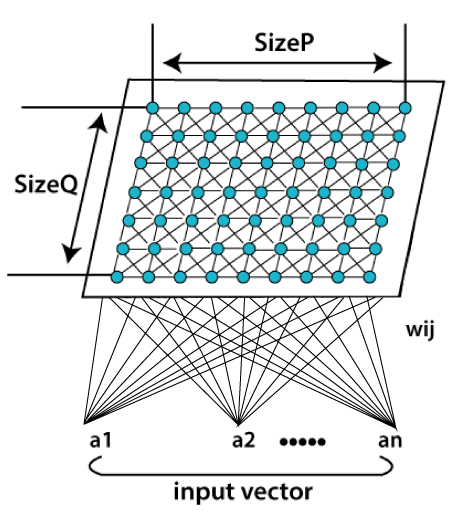
\includegraphics[width=0.3\linewidth]{pics/som_example_diapo_1.png}
				\caption{SOM Architecture (see 2 of Bibliography).}
			\end{figure}
		\end{center}

		\end{block}		

		\begin{block}{Wikipedia}

A self-organizing map (SOM) is used to produce a low-dimensional (typically two-dimensional) representation of a higher dimensional data set, while preserving the topological structure of the data. 
		\end{block}
	\end{frame}
	
	
	\begin{frame}{Motivation}

		The Self-Organizing Maps permit to : 

		\begin{itemize}
		
			\item Analyse and visualise the data. It represents complex data on a map of only two or three dimensions (see Convergence slide).

			\item Detect patterns from the data. Clustering (see K-means slide).

			\item Improve a deep neuronal network by sorting the data at the beginning.

		\end{itemize}


	\end{frame}
	

	\begin{frame}{Example}
  
		\begin{columns}
    
			\begin{column}{0.33\textwidth}
      
				\centering
				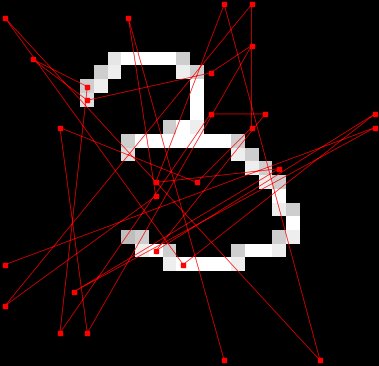
\includegraphics[width=1\textwidth]{pics/algo_1_1.png}
Step 1
    			\end{column}

    				
			\begin{column}{0.33\textwidth}
      
				\centering
				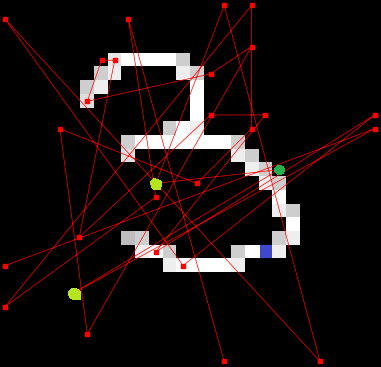
\includegraphics[width=1\textwidth]{pics/algo_1_2.png}
Step 2
    			\end{column}

    
			\begin{column}{0.33\textwidth}
      
				\centering
      				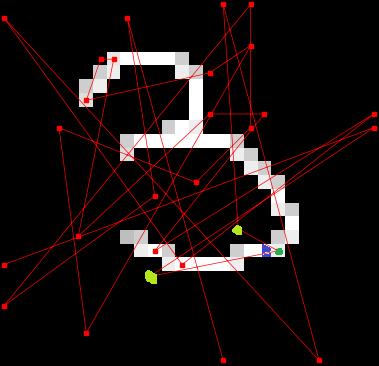
\includegraphics[width=1\textwidth]{pics/algo_1_3.png}
Step 3
    			\end{column}
		\end{columns}




               	\begin{enumerate}

                        \item Initialize the weight vectors (randomly or not) in red.
			\item \textbf{Competition} : Select a data vector(blue), then chose the closest weight vector(green) to it.
			\item \textbf{Adaptation} : Update the winner and its neighbors (all green ones).
                        \item repeat the process till reach max$\textunderscore$iteration
                \end{enumerate}
        \end{frame}


	\begin{frame}{Similarities with the Perceptron}
	
		\begin{block}{Perceptron}

			\begin{center}
				
				\begin{figure}[h]

					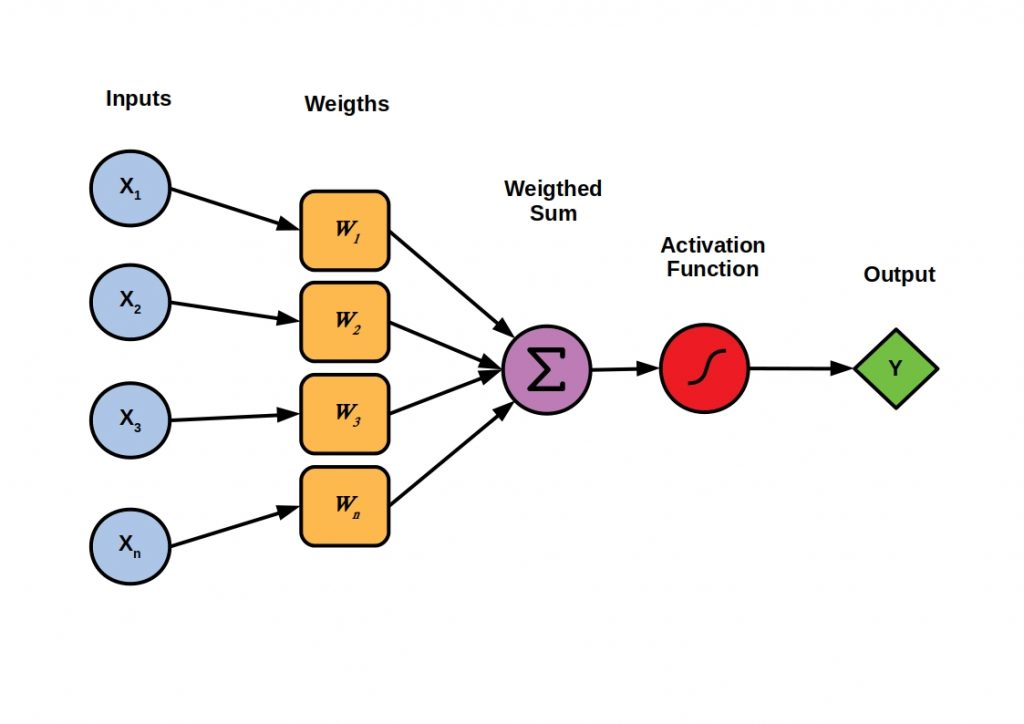
\includegraphics[width=0.4\linewidth]{pics/Perceptrons-1024x724.jpeg}
					\caption{Diagram of a Perceptron.}	
				\end{figure}
			\end{center}

			It is also a one-layer neuronal network. However, this one is used to separate two different classes. The output is actually a binary one. 

			This is a supervised learning algorithm.
		\end{block}

		
		\begin{block}{SOM}
		
			The SOM can gather vectors due to their similarities.

			The SOM is an \textbf{unsupervised learning algorithm}.
		\end{block}



	\end{frame}
	
	
	\begin{frame}{Similarities with K-means algorithm}
		
		K-means algorithm is an unsupervised learning technique that can automatically gather data by creating \textbf{clusters}, which are subsets of data elements that share common characteristics.

		\begin{center}
			
			\begin{figure}[h]
			
				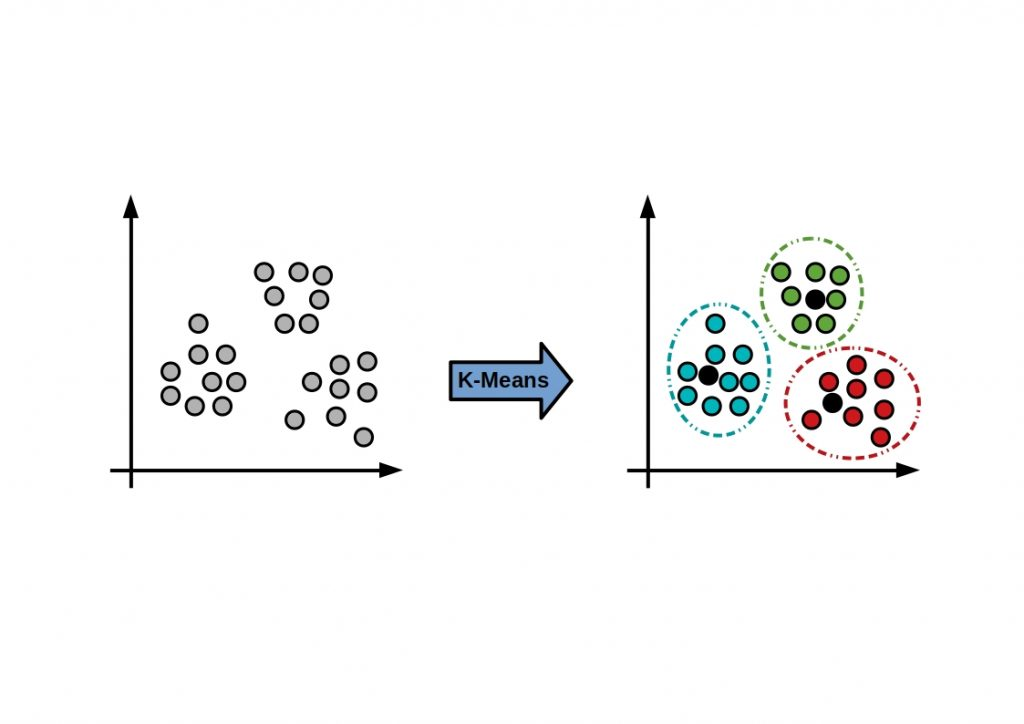
\includegraphics[width=0.6\linewidth]{pics/kmeans.jpeg}
				\caption{Process of K-means algorithm}
			\end{figure}
		\end{center}
				
		The user must define the number of clusters \textbf{K}. However, The SOM does not require this, it guesses the right amount of clusters.

	\end{frame}

	
	\begin{frame}{Convergence}
		
		The convergence of the SOM algorithm is not guaranteed (1). There are actually 2 errors that can appear.

                     
		\begin{columns}
                        
                        \column{0.5\textwidth}
                
                        	\begin{figure}[h]
                
                                	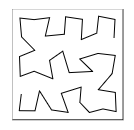
\includegraphics[width=0.5\linewidth]{pics/dimension_error.png}
					\caption{\tiny \textbf{Dimension Error}. 

It happens when the number of neurons does not fit with the data. 

The ideal number of neurons is 5$\sqrt{N}$ where N is the number of data vectors.}
                        	\end{figure}
                        
                        
                        \column{0.5\textwidth}
                        
                        	\begin{figure}[h]
                                
                                	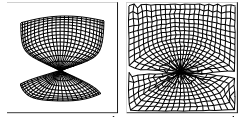
\includegraphics[width=0.5\linewidth]{pics/topological_error.png} 
					\caption{\tiny \textbf{Topological Error}. 

It happens when a node is created. It looks like a butterfly.}             
                        	\end{figure}
		\end{columns}
	\end{frame}



\section{Algorithm}

	\begin{frame}
	
		\begin{center}
			
			\Huge ALGORITHM
		\end{center}
	\end{frame}


	\begin{frame}{Different Phases}

		\begin{columns}

			\begin{column}{0.7\textwidth}

				\begin{block}{Initialisation}

The weights $m_i$ or $w_i$ of neuron connections are randomly initialized.
				\end{block}


				\begin{block}{Competition}
		
Chose randomly an input vector $X_j$. 

Search for the neuron with the closest weight vector from $X_j$.

To realise it, a distance is needed. 

All distances can work, let is choose the \textbf{Euclidean distance}. 

The identity of the \textbf{winner} neuron is : 

					\begin{center}
		
						k = $\arg\limits_{i} \min \| X_j - w_i \|$
					\end{center}
				\end{block}
			\end{column}

			\begin{column}{0.4\textwidth}
				
				\begin{center}
					
					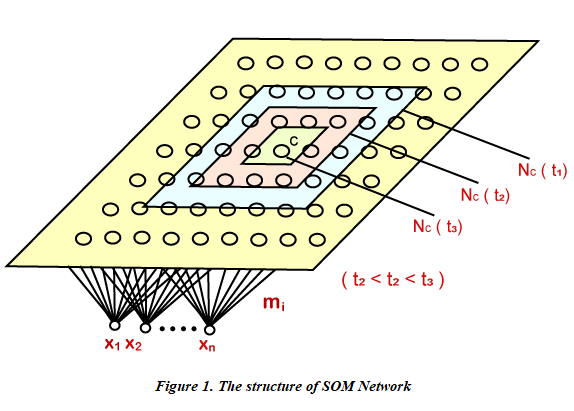
\includegraphics[width=1\linewidth]{pics/explanation_phases.png}	
				\end{center}
			\end{column}
		\end{columns}
	\end{frame}

		
	\begin{frame}{Cooperation}

To prevent from discontinous adaptation by only modifying the winner neuron, all of its neighbors are also modified.

The number of neighbors depends on the topology.
		\begin{center}
			
			\begin{figure}[h]
			
				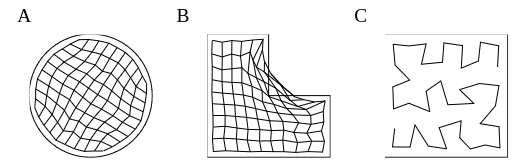
\includegraphics[width=0.5\linewidth]{pics/topologies.png}
				\caption{\tiny \textbf{Different topologies possible}.



A : circular topology;  

B : rectangular topology;  

C : linear topology
}
			\end{figure}
		\end{center}
		

Here, the grid is the neural network.

Each node of the grid is a neuron.

On the linear topology, each neuron has a maximum number of 2 neighbors.

On the rectangular topology, each neuron has a maximum number of 8 neighbors.
	\end{frame}


	\begin{frame}{Adaptation}

Here is the update of the weight vectors of the winner neuron and its neighbors.

it is at the instant t : 

		\begin{center}

			$w_k$(t + 1) = $w_k$(t) + $\alpha$.$h_{kj}$(t).($X_j$ - $w_k$(t))	
		\end{center}

		\begin{itemize}
	
			\item $X_j$ is the input vector
			\item $w_k$(t) is the weight vector of the neuron k at the instant t
			\item $\alpha$ is the \textbf{learning rate}
			\item $h_{kj}$ is the \textbf{neighborhood} function which smooths the update of the neighbors depending on their proximity with the winner and the iteration t. (see 1 of Bibliography)
		\end{itemize}
	
We can chose the \textbf{Gaussian} function :

			\begin{center}
		
				$h_{jk}$ = exp($\frac{-\|w_{winner} - w_k\|^2}{2\sigma^2}$)
			\end{center}
		
$\sigma$ is the standard deviation of the Gaussian function (2). It could be a function which decreases with t.
	\end{frame}


	\begin{frame}{Algorithm}

		\begin{columns}

			\column{0.6\textwidth}

				\begin{algorithm}[H]
			
					\caption{Self-Organizing Map Algorithm}
					\begin{algorithmic}[1]		
					
						\REQUIRE input data \textbf{X}; maximum number of iterations \textbf{IMAX}; the neighborhood function \textbf{h}; lattice dimensions \textbf{k}x\textbf{l}
			
						\ENSURE the weight vectors \textbf{W}
						
						\STATE Randomly initialize weight vectors $w_i$	
									
						 \FOR{t $\leftarrow$ 1 \textbf{to} IMAX} 

						 \STATE {

							 \FOR{sample \textbf{in} X}

							\STATE {
								
								\textit{competition}
			
								\STATE Find the neuron closest to the sample
								
								\textit{cooperation and adaptation}

								\STATE Find this neuron and its neighbors
							} \ENDFOR
						 } \ENDFOR
				
						\RETURN W
					\end{algorithmic}
				\end{algorithm}
		\end{columns}
	\end{frame}
	


\section{Bibliography}
	
	\begin{frame}
	
		\begin{center}

			\Huge BIBLIOGRAPHY
		\end{center}
	\end{frame}


	\begin{frame}
	
		\begin{enumerate}
			
			\item Self-Organizing Maps - Teuvo Kohonen (2001)
			\item https://www.baeldung.com/cs/som-algorithm
			\item http://www.pspc.unige.it/~drivsco/Papers/VanHulle$\textunderscore$Springer.pdf
		\end{enumerate}
	\end{frame}





\end{document}
